\chapter{Filters}

\section{Introduction}

\subsection{Key Concepts}

glscopeclient and libscopehal are based on a ``filter graph" architecture internally. The filter graph is a directed
acyclic graph with a set of source nodes (waveforms captured from hardware, loaded from a saved session, or generated
numerically) and sink nodes (waveform views, protocol analyzer views, and statistics) connected by edges representing
data flow.

A filter is simply an intermediate node in the graph, which takes input from zero or more waveform nodes and outputs a
waveform which may be displayed, used as input to other filters, or both. A waveform is a series of data points which
may represent voltages, digital samples, or arbitrarily complex protocol data structures.

As a result, there is no internal distinction between math functions, measurements, and protocol decodes, and it is
possible to chain them arbitrarily. Consider the following example:

\begin{itemize}
\item Two analog waveforms representing serial data and clock are acquired
\item Each analog waveform is thresholded, producing a digital waveform
\item The two digital waveforms are decoded as $I^2C$, producing a series of packets
\item The $I^2C$ packets are decoded as writes to a serial DAC, producing an analog waveform
\item A moving average filter is applied to the analog waveform
\item A measurement filter finds the instantaneous frequency of each cycle of the DAC output
\end{itemize}

In this document we use the term ``filter" consistently to avoid ambiguity.

\subsection{Conventions}

A filter can take arbitrarily many inputs (vector inputs), arbitrarily many parameters (scalar inputs), and outputs a
signal (vector output).

If the output signal is a multi-field type (as opposed to a single scalar, e.g. voltage, at each sample) the
``Output Signal" section will include a table describing how various types of output data are displayed. Printf-style
format codes maybe used for clarity. For example, ``\%02x" means data is formatted as hexadecimal bytes with leading
zeroes.

All filters with complex output use a standardized set of colors to display various types of data fields in a
consistent manner. These colors are configurable under the \menustyle{Appearance / Decodes} preferences category.

\begin{tabularx}{16cm}{llX}
\thickhline
\textbf{Color name} & \textbf{Use case} & \textbf{Default Color} \\
\thickhline
Address & Memory addresses & \cellcolor{address}\textcolor{black}{\#ffff00} \\
\thickhline
Checksum Bad & Incorrect CRC/checksum & \cellcolor{checksumbad}\textcolor{white}{\#ff0000} \\
\thickhline
Checksum OK & Valid CRC/checksum & \cellcolor{checksumok}\textcolor{black}{\#00ff00} \\
\thickhline
Control & Miscellaneous control data & \cellcolor{control}\textcolor{white}{\#c000a0} \\
\thickhline
Data & User data & \cellcolor{data}\textcolor{white}{\#336699} \\
\thickhline
Error & Malformed/unreadable data & \cellcolor{error}\textcolor{white}{\#ff0000} \\
\thickhline
Idle & Inter-frame gaps & \cellcolor{idle}\textcolor{white}{\#404040} \\
\thickhline
Preamble & Preamble/sync words & \cellcolor{preamble}\textcolor{white}{\#808080} \\
\thickhline
\end{tabularx}

%%%%%%%%%%%%%%%%%%%%%%%%%%%%%%%%%%%%%%%%%%%%%%%%%%%%%%%%%%%%%%%%%%%%%%%%%%%%%%%%%%%%%%%%%%%%%%%%%%%%%%%%%%%%%%%%%%%%%%%%
\pagebreak
\section{64b/66b}
\label{filter:64b66b}

Decodes the 64/66b line code used by \hyperref[filter:10gbaser]{10Gbase-R} and other serial protocols, as originally
specified in IEEE 802.3 clause 49.2.

64b/66b is a serial line code which divides transmitted data into 64-bit blocks and scrambles them with a LFSR, then
appends a 2-bit type field (which is not scrambled) to each block for synchronization. Block synchronization depends on
always having an edge in the type field so types 2'b00 and 2'b11 are disallowed.

Note that this filter only performs block alignment and descrambling. No decoding is applied to the 64-bit blocks, as
different upper-layer protocols assign different meaning to them. In 10Gbase-R, type 2'b01 denotes ``64 bits of upper
layer data" and type 2'b10 denotes ``8-bit type field and 56 bits of data whose meaning depends on the type", however
this is not universal.

\begin{figure}[h]
\centering
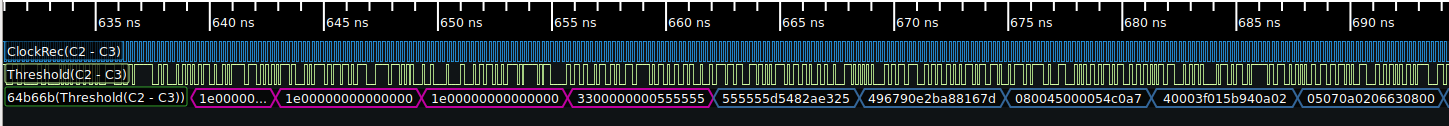
\includegraphics[width=16cm]{images/filters/64b66b.png}
\caption{Example 64b/66b decode}
\label{filter_64b66b}
\end{figure}

\subsection{Inputs}

\begin{tabularx}{16cm}{llX}
\thickhline
\textbf{Signal name} & \textbf{Type} & \textbf{Description} \\
\thickhline
data & 1-bit digital & Serial 8b/10b data line \\
\thickhline
clk & 1-bit digital & DDR bit clock, typically generated by use of the \hyperref[filter:cdrpll]{Clock Recovery
(PLL)} filter on the input data.\\
\thickhline
\end{tabularx}

\subsection{Parameters}

This filter takes no parameters.

\subsection{Output Signal}

The 64B/66B filter outputs a time series of 64B/66B sample objects. These consist of a control/data flag and
a 64-bit data block.

\begin{tabularx}{16cm}{lllX}
\thickhline
\textbf{Type} & \textbf{Description} & \textbf{Color} & \textbf{Format} \\
\thickhline
Control & Block with type 2'b10 & \cellcolor{control}\textcolor{white}{Control} & \%016x \\
\thickhline
Data & Block with type 2'b01 & \cellcolor{data}\textcolor{white}{Data} & \%016x \\
\thickhline
Error & Block with type 2'b00 or 2'b11 & \cellcolor{error}\textcolor{white}{Error} & \%016x \\
\thickhline
\end{tabularx}

%%%%%%%%%%%%%%%%%%%%%%%%%%%%%%%%%%%%%%%%%%%%%%%%%%%%%%%%%%%%%%%%%%%%%%%%%%%%%%%%%%%%%%%%%%%%%%%%%%%%%%%%%%%%%%%%%%%%%%%%
\pagebreak
\section{8B/10B (IBM)}
\label{filter:8b10b}

Decodes the standard 8b/10b line code used by SGMII, \hyperref[filter:1000basex]{1000base-X}, DisplayPort, JESD204,
\hyperref[filter:pcie2_logical]{PCIe gen 1/2}, SATA, USB 3.0, and many other common serial protocols.

8b/10b is a dictionary based code which converts each byte of message data to a ten-bit code. In order to maintain DC
balance and limit run length to a maximum of five identical bits in a row, all legal codes have one of:
\begin{itemize}
\item One legal coding, with exactly five zero bits
\item Two legal codings, one with four zero bits and one with six
\end{itemize}

The transmitter maintains a ``running disparity" counter and chooses the appropriate coding for each symbol to ensure
DC balance. There are twelve legal codes which are not needed for encoding data values; these are used to encode
frame boundaries, idle/alignment sequences, and other control information.

\begin{figure}[h]
\centering
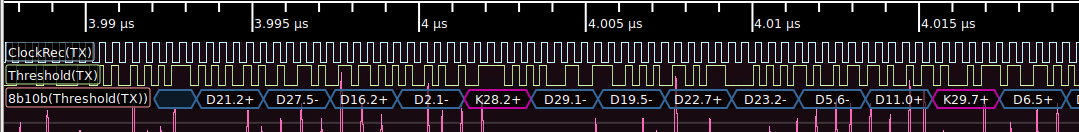
\includegraphics[width=16cm]{images/filters/8b10b.png}
\caption{Example 8b/10b decode}
\label{filter_8b10b}
\end{figure}

\subsection{Inputs}

\begin{tabularx}{16cm}{llX}
\thickhline
\textbf{Signal name} & \textbf{Type} & \textbf{Description} \\
\thickhline
data & 1-bit digital & Serial 8b/10b data line \\
\thickhline
clk & 1-bit digital & DDR bit clock, typically generated by use of the \hyperref[filter:cdrpll]{Clock Recovery
(PLL)} filter on the input data.\\
\thickhline
\end{tabularx}

\subsection{Parameters}

\begin{tabularx}{16cm}{llX}
\thickhline
\textbf{Parameter name} & \textbf{Type} & \textbf{Description} \\
\thickhline
Display Format & Enum &
	\textbf{Dotted (K28.5 D21.5)}: displays the 3b4b and 5b6b code blocks separately, with K or D prefix. \newline
	\textbf{Hex (K.bc b5)}: displays data as hex byte values and control codes with a K prefix. \\
\thickhline
\end{tabularx}

\subsection{Output Signal}

The 8B/10B filter outputs a time series of 8B/10B sample objects. These consist of a control/data flag and a byte of
data.

\begin{tabularx}{16cm}{lllX}
\thickhline
\textbf{Type} & \textbf{Description} & \textbf{Color} & \textbf{Format} \\
\thickhline
Control & Control codes & \cellcolor{control}\textcolor{white}{Control} & K\%d.\%d+ \\
\thickhline
Data & Upper layer protocol data & \cellcolor{data}\textcolor{white}{Data} & D\%d.\%d+ \\
\thickhline
Error & Malformed data & \cellcolor{error}\textcolor{white}{Error} & ERROR \\
\thickhline
\end{tabularx}

%%%%%%%%%%%%%%%%%%%%%%%%%%%%%%%%%%%%%%%%%%%%%%%%%%%%%%%%%%%%%%%%%%%%%%%%%%%%%%%%%%%%%%%%%%%%%%%%%%%%%%%%%%%%%%%%%%%%%%%%
\pagebreak
\section{8B/10B (TMDS)}
\label{filter:tmds}

Decodes the 8-to-10 Transition Minimized Differential Signalling line code used in \hyperref[filter:dvi]{DVI} and HDMI.

Like the \hyperref[filter:8b10b]{8B/10B (IBM)} line code, TMDS is an 8-to-10 bit serial line code. TMDS, however, is
designed to \emph{minimize} the number of toggles in the data stream for EMC reasons, rendering it difficult to
synchronize a CDR PLL to. As a result, HDMI and DVI provide a reference clock at the pixel clock rate (1/10 the serial
data bit rate) along with the data stream to provide synchronization.

\begin{figure}[h]
\centering
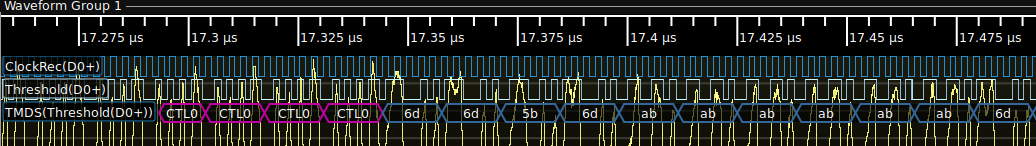
\includegraphics[width=16cm]{images/filters/tmds.png}
\caption{Example TMDS decode}
\label{filter_tmds}
\end{figure}

\subsection{Inputs}

\begin{tabularx}{16cm}{llX}
\thickhline
\textbf{Signal name} & \textbf{Type} & \textbf{Description} \\
\thickhline
data & 1-bit digital & Serial TMDS data line \\
\thickhline
clk & 1-bit digital & DDR \emph{bit} clock, typically generated by use of the \hyperref[filter:cdrpll]{Clock Recovery
(PLL)} filter on the input data. Note that this is 5x the rate of the pixel clock signal. \\
\thickhline
\end{tabularx}

\subsection{Parameters}

\begin{tabularx}{16cm}{llX}
\thickhline
\textbf{Parameter name} & \textbf{Type} & \textbf{Description} \\
\thickhline
Lane Number & Integer & Lane number within the link (0-3)\\
\thickhline
\end{tabularx}

\subsection{Output Signal}

The TMDS filter outputs a time series of TMDS sample objects. These consist of a type field and a byte of data.

The output of the TMDS decode is commonly fed to the \hyperref[filter:dvi]{DVI} or \hyperref[filter:hdmi]{HDMI}
protocol decoders.

\begin{tabularx}{16cm}{lllX}
\thickhline
\textbf{Type} & \textbf{Description} & \textbf{Color} & \textbf{Format} \\
\thickhline
Control & Control codes (H/V sync) & \cellcolor{control}\textcolor{white}{Control} & CTL\%d \\
\thickhline
Data & Pixel/island data & \cellcolor{data}\textcolor{white}{Data} & \%02x \\
\thickhline
Error & Malformed data & \cellcolor{error}\textcolor{white}{Error} & ERROR \\
\thickhline
Guard band & HDMI data/video guard band & \cellcolor{preamble}\textcolor{white}{Preamble} & GB \\
\thickhline
\end{tabularx}

%%%%%%%%%%%%%%%%%%%%%%%%%%%%%%%%%%%%%%%%%%%%%%%%%%%%%%%%%%%%%%%%%%%%%%%%%%%%%%%%%%%%%%%%%%%%%%%%%%%%%%%%%%%%%%%%%%%%%%%%
\pagebreak
\section{AC Couple}
\label{filter:accouple}

Automatically removes a DC offset from an analog waveform by subtracting the average of all samples from each sample.

This filter should only be used in postprocessing already acquired data, or other situations in which AC coupling in
the hardware (via an AC coupled probe, or coaxial DC block) is not possible.

\begin{figure}[h]
\centering
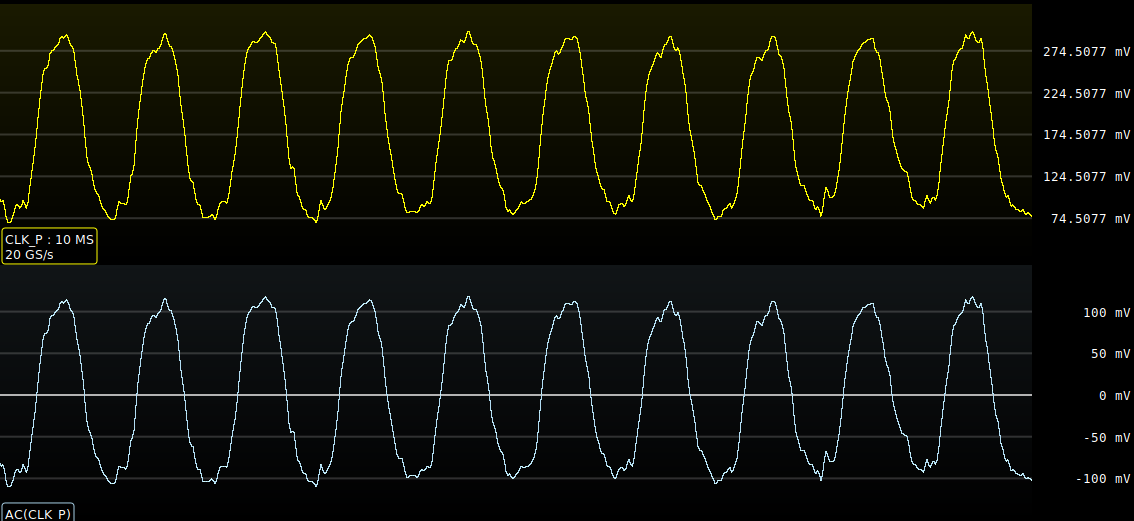
\includegraphics[width=16cm]{images/filters/ac-couple.png}
\caption{Example AC coupling}
\end{figure}

\subsection{Inputs}

\begin{tabularx}{16cm}{llX}
\thickhline
\textbf{Signal name} & \textbf{Type} & \textbf{Description} \\
\thickhline
din & Analog & Input waveform \\
\thickhline
\end{tabularx}

\subsection{Parameters}

This filter takes no parameters.

\subsection{Output Signal}

This filter outputs an analog waveform with identical sample rate to the input, vertically shifted to center the signal
at zero volts.

%%%%%%%%%%%%%%%%%%%%%%%%%%%%%%%%%%%%%%%%%%%%%%%%%%%%%%%%%%%%%%%%%%%%%%%%%%%%%%%%%%%%%%%%%%%%%%%%%%%%%%%%%%%%%%%%%%%%%%%%
\pagebreak
\section{ADL5205}
\label{filter:adl5205}

Decodes SPI data traffic to one half of an ADL5205 variable gain amplifier.

TODO: Screenshot

\subsection{Inputs}

\begin{tabularx}{16cm}{llX}
\thickhline
\textbf{Signal name} & \textbf{Type} & \textbf{Description} \\
\thickhline
spi & SPI bus & The SPI data bus \\
\thickhline
\end{tabularx}

\subsection{Parameters}

This filter takes no parameters.

\subsection{Output Signal}

This filter outputs one ADL5205 sample object for each write transaction, formatted as ``write: FA=2 dB, gain=8 dB".

%%%%%%%%%%%%%%%%%%%%%%%%%%%%%%%%%%%%%%%%%%%%%%%%%%%%%%%%%%%%%%%%%%%%%%%%%%%%%%%%%%%%%%%%%%%%%%%%%%%%%%%%%%%%%%%%%%%%%%%%
\pagebreak
\section{Autocorrelation}
\label{filter:autocorrelation}

This filter calculates the autocorrelation of an analog waveform. Autocorrelation is a measure of self-similarity
calculated by multiplying the signal with a time-shifted copy of itself. In Fig. \ref{filter_accouple}, strong peaks
can be seen at multiples of the 8b/10b symbol rate.

For best performance, it is crucial to keep the maximum offset as low as possible, since filter run time grows linearly
with offset range.

\begin{figure}[h]
\centering
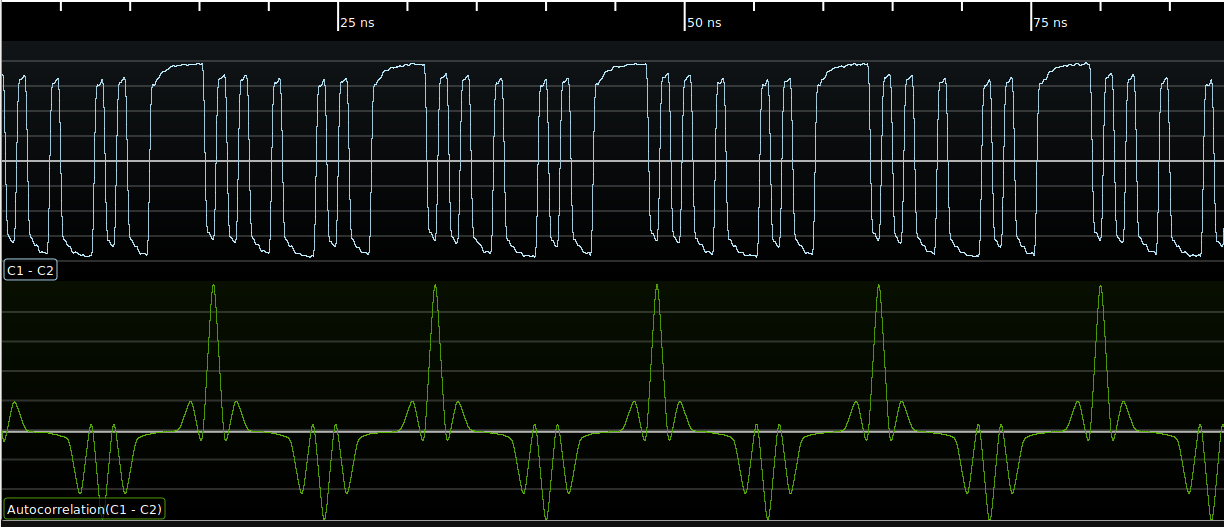
\includegraphics[width=16cm]{images/filters/autocorrelation.png}
\caption{Example of autocorrelation on a serial data stream}
\label{filter_accouple}
\end{figure}

\subsection{Inputs}

\begin{tabularx}{16cm}{llX}
\thickhline
\textbf{Signal name} & \textbf{Type} & \textbf{Description} \\
\thickhline
din & Analog & Input waveform \\
\thickhline
\end{tabularx}

\subsection{Parameters}

\begin{tabularx}{16cm}{llX}
\thickhline
\textbf{Parameter name} & \textbf{Type} & \textbf{Description} \\
\thickhline
Max offset & Integer & Maximum shift (in samples)\\
\thickhline
\end{tabularx}

\subsection{Output Signal}

This filter outputs an analog waveform with the same timebase as the input, one sample for each correlation offset.

%%%%%%%%%%%%%%%%%%%%%%%%%%%%%%%%%%%%%%%%%%%%%%%%%%%%%%%%%%%%%%%%%%%%%%%%%%%%%%%%%%%%%%%%%%%%%%%%%%%%%%%%%%%%%%%%%%%%%%%%
\pagebreak
\section{Base}
\label{filter:base}

Calculates the base (logical zero level) of each cycle in a digital waveform.

It is most commonly used as an input to statistics, to view the average base of the entire waveform. At times, however,
it may be useful to view the base waveform. For example, in Fig. \ref{filter_base}, the vertical eye closure caused by
channel ISI is readily apparent.

\begin{figure}[h]
\centering
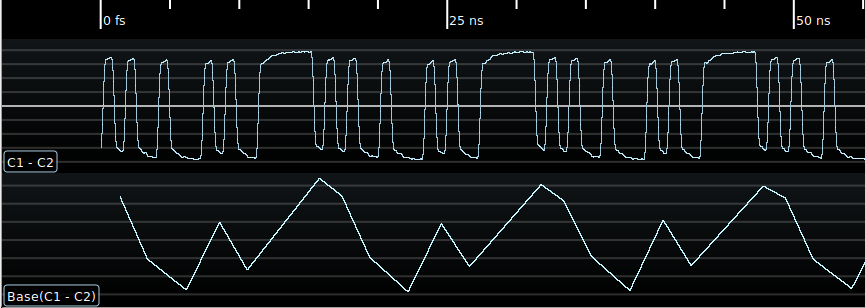
\includegraphics[width=16cm]{images/filters/base.png}
\caption{Example of base measurement on a serial data stream}
\label{filter_base}
\end{figure}

\subsection{Inputs}

\begin{tabularx}{16cm}{llX}
\thickhline
\textbf{Signal name} & \textbf{Type} & \textbf{Description} \\
\thickhline
din & Analog & Input waveform \\
\thickhline
\end{tabularx}

\subsection{Parameters}

This filter takes no parameters.

\subsection{Output Signal}

This filter outputs an analog waveform with one sample for each group of logical zeroes in the input signal, containing
the average value of the zero level for the middle 50\% of the low period.

%%%%%%%%%%%%%%%%%%%%%%%%%%%%%%%%%%%%%%%%%%%%%%%%%%%%%%%%%%%%%%%%%%%%%%%%%%%%%%%%%%%%%%%%%%%%%%%%%%%%%%%%%%%%%%%%%%%%%%%%
\pagebreak
\section{CAN}
\label{filter:can}

Decodes the Control Area Network (CAN) bus, commonly used in vehicle control systems. Both standard (11 bit) and
extended (29 bit) IDs are supported.

CAN-FD frames are detected and flagged as such, but the current decode cannot parse them fully.

\begin{figure}[h]
\centering
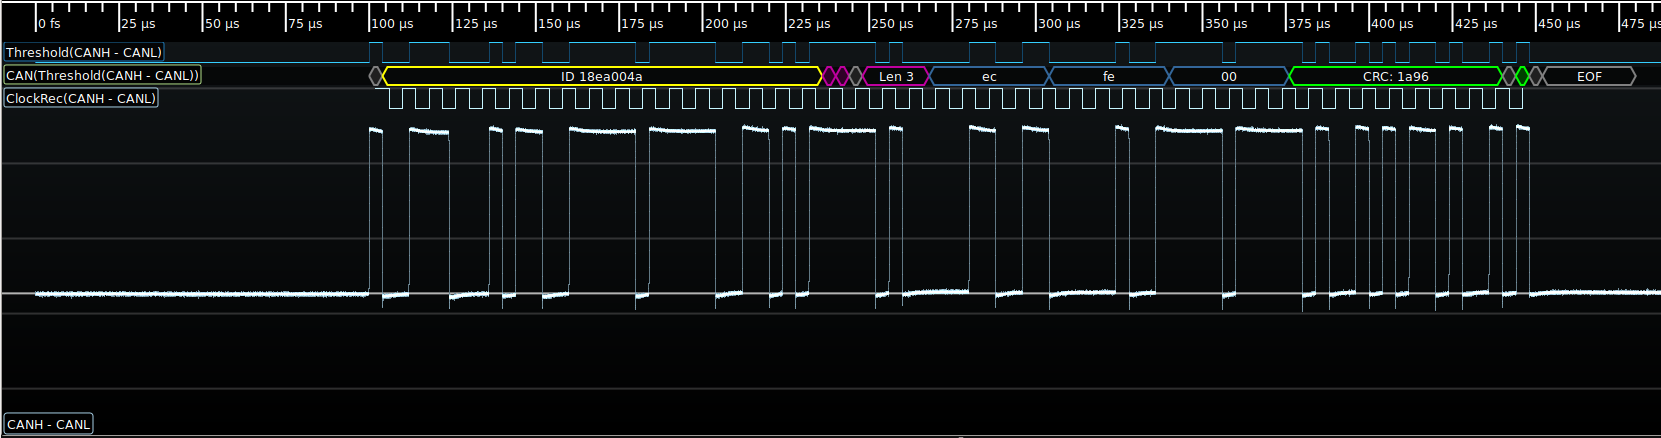
\includegraphics[width=16cm]{images/filters/can.png}
\caption{Example of CAN bus protocol decode}
\label{filter_can}
\end{figure}

\subsection{Inputs}

\begin{tabularx}{16cm}{llX}
\thickhline
\textbf{Signal name} & \textbf{Type} & \textbf{Description} \\
\thickhline
CANH & Digital & Thresholded CANH (or CANH-CANL) signal \\
\thickhline
\end{tabularx}

\subsection{Parameters}

\begin{tabularx}{16cm}{llX}
\thickhline
\textbf{Parameter name} & \textbf{Type} & \textbf{Description} \\
\thickhline
Bit Rate & Integer & Bit rate of the bus (most commonly 250 or 500 Kbps)\\
\thickhline
\end{tabularx}

\subsection{Output Signal}

The CAN bus decode outputs a time series of CAN sample objects. These consist of a type field and a byte of data.

\begin{tabularx}{16cm}{lllX}
\thickhline
\textbf{Type} & \textbf{Description} & \textbf{Color} & \textbf{Format} \\
\thickhline
Control & Start of frame & \cellcolor{preamble}\textcolor{white}{Preamble} & SOF \\
\thickhline
ID & CAN ID & \cellcolor{address}\textcolor{black}{Address} & ID \%x \\
\thickhline
RTR & Remote Transmission Request & \cellcolor{control}\textcolor{white}{Control} & DATA | REQ \\
\thickhline
FD mode & CAN-FD mode & \cellcolor{control}\textcolor{white}{Control} & FD | STD\\
\thickhline
R0 & Reserved bits & \cellcolor{preamble}\textcolor{white}{Preamble} & RSVD \\
\thickhline
DLC & Data Length Code & \cellcolor{control}\textcolor{white}{Control} & Len 3 \\
\thickhline
Data & Payload data & \cellcolor{data}\textcolor{white}{Data} & \%02x \\
\thickhline
Valid CRC & Good checksum & \cellcolor{checksumok}\textcolor{black}{Checksum OK} & CRC: \%04x \\
\thickhline
Invalid CRC & Bad checksum & \cellcolor{checksumbad}\textcolor{white}{Checksum Bad} & CRC: \%04x \\
\thickhline
CRC delimiter & Bus turnaround & \cellcolor{preamble}\textcolor{white}{Preamble} & CRC DELIM \\
\thickhline
ACK & Acknowledgement & \cellcolor{checksumok}\textcolor{black}{Checksum OK} & ACK \\
\thickhline
NAK & Missing acknowledgement & \cellcolor{checksumbad}\textcolor{white}{Checksum Bad} & NAK \\
\thickhline
ACK delimiter & Bus turnaround & \cellcolor{preamble}\textcolor{white}{Preamble} & ACK DELIM \\
\thickhline
EOF & End of frame & \cellcolor{preamble}\textcolor{white}{Preamble} & EOF \\

\thickhline
\end{tabularx}

%%%%%%%%%%%%%%%%%%%%%%%%%%%%%%%%%%%%%%%%%%%%%%%%%%%%%%%%%%%%%%%%%%%%%%%%%%%%%%%%%%%%%%%%%%%%%%%%%%%%%%%%%%%%%%%%%%%%%%%%
\pagebreak
\section{Channel Emulation}
\label{filter:channelemu}

This filter models the effects of applying an arbitrary channel, described via a set of 2-port S-parameters, to
a waveform. Fig. \ref{filter_channelemu} shows the result of passing a 1.25 Gbps serial data pattern through a 10x
oscilloscope probe with approximately 500 MHz bandwidth. The ISI, attenuation, and phase shift introduced by the
channel can all be seen.

The channel model works in the frequency domain. An FFT is performed on the input, then each complex point is scaled by
the interpolated magnitude and rotated by the phase, then an inverse FFT is used to transform the signal back into the
time domain.

The group delay of the channel is then estimated and samples are discarded from the beginning of the waveform to
prevent causality violations. For example, when performing channel emulation using a network with a 1ns group delay,
the output waveform will begin 1ns after the input (since the channel output before this depends on input samples
before the start of the waveform). Note that the automatic group delay estimation uses points from roughly the center
of the S-parameter dataset in the current implementation; channels which do not have a significant passband around this
frequency will give incorrect group delay estimates. The ``Group Delay Truncation Mode" parameter can be set to manual
in this case, selecting the ``Group Delay Truncation" parameter instead of the automatically estimated value.

\begin{figure}[h]
\centering
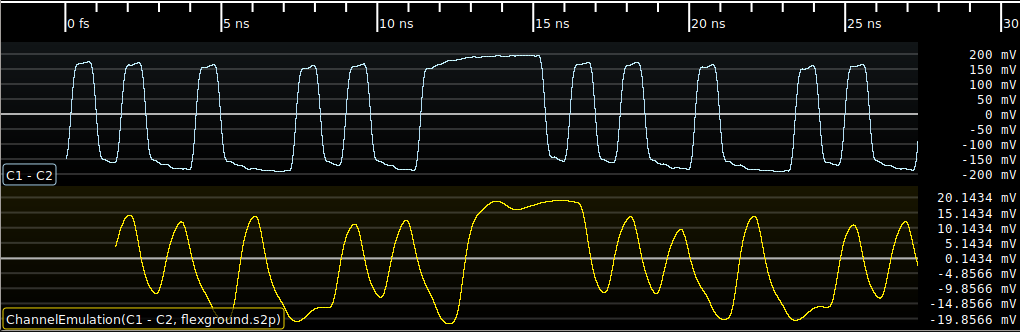
\includegraphics[width=16cm]{images/filters/channel-emulation.png}
\caption{Example of channel emulation on a serial data stream}
\label{filter_channelemu}
\end{figure}

\subsection{Inputs}

\begin{tabularx}{16cm}{llX}
\thickhline
\textbf{Signal name} & \textbf{Type} & \textbf{Description} \\
\thickhline
signal & Analog & Input waveform \\
\thinhline
mag & Analog & S-parameter magnitude channel \\
\thinhline
ang & Analog & S-parameter angle channel \\
\thickhline
\end{tabularx}

\subsection{Parameters}

\begin{tabularx}{16cm}{llX}
\thickhline
\textbf{Parameter name} & \textbf{Type} & \textbf{Description} \\
\thickhline
Max Gain & Float & Maximum gain to apply\\
\thinhline
Group Delay Truncation & Int & Group delay override for manual mode\\
\thinhline
Group Delay Truncation Mode & Enum & Specifies manual or automatically estimated group delay\\
\thickhline
\end{tabularx}

\subsection{Output Signal}

This filter outputs an analog waveform with the same timebase as the input, with the emulated channel applied.

%%%%%%%%%%%%%%%%%%%%%%%%%%%%%%%%%%%%%%%%%%%%%%%%%%%%%%%%%%%%%%%%%%%%%%%%%%%%%%%%%%%%%%%%%%%%%%%%%%%%%%%%%%%%%%%%%%%%%%%%
\pagebreak
\section{Clock Recovery (D-PHY HS Mode)}

Extracts a double-rate clock from a MIPI D-PHY clock+data stream, which is gated to only toggle when the data input
is in HS mode. This can be used for generating eye patterns of the HS-mode data.

%%%%%%%%%%%%%%%%%%%%%%%%%%%%%%%%%%%%%%%%%%%%%%%%%%%%%%%%%%%%%%%%%%%%%%%%%%%%%%%%%%%%%%%%%%%%%%%%%%%%%%%%%%%%%%%%%%%%%%%%
\pagebreak
\section{Clock Recovery (PLL)}
\label{filter:cdrpll}

This filter uses a PLL to recover a clock from a serial data stream. The recovered clock is double-rate and
phased 90\textdegree with respect to the data, such that the data can be sampled directly by both edges of the PLL
output clock.

When the optional clock gating input is low, the output does not toggle and any edges in the input signal are ignored.
As soon as the gate goes high, the PLL will phase shift the internal NCO to align with the next transition in the input
signal and then begin running closed-loop.

NOTE: The current edge detector uses a single threshold suitable for NRZ inputs. When using a multi-level modulation
such as PAM-4 or MLT-3, set the threshold to the highest or lowest crossing level. This will work fine for MLT-3 but
introduces some data-dependent jitter in PAM signals (since the slew rate for an 00-11 transition is different than
that for a 10-11 transition). The resulting recovered clock should still be adequate for protocol decoding, however a
better edge detector will need to be implemented in order to do adequate jitter measurements on PAM waveforms.

\begin{figure}[h]
\centering
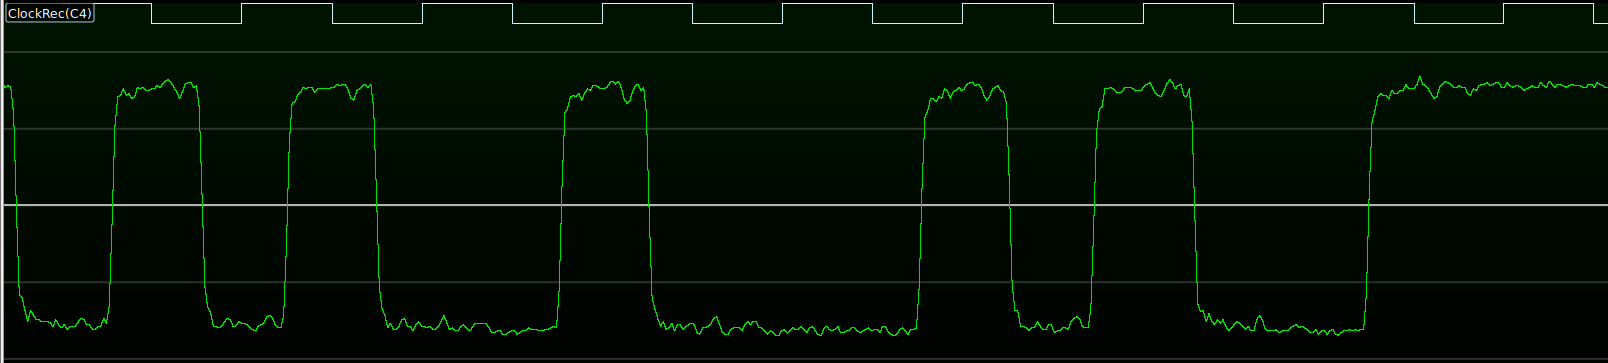
\includegraphics[width=16cm]{images/filters/cdrpll.png}
\caption{Example of CDR PLL on a serial data stream}
\label{filter_cdrpll}
\end{figure}

\subsection{Inputs}

\begin{tabularx}{16cm}{llX}
\thickhline
\textbf{Signal name} & \textbf{Type} & \textbf{Description} \\
\thickhline
IN & Analog & Input waveform \\
\thinhline
Gate & Digital & Clock enable signal, or NULL to disable gating\\
\thickhline
\end{tabularx}

\subsection{Parameters}

\begin{tabularx}{16cm}{llX}
\thickhline
\textbf{Parameter name} & \textbf{Type} & \textbf{Description} \\
\thickhline
Symbol rate & Float & Symbol rate, in Hz\\
\thinhline
Threshold & Float & Decision threshold for the edge detector, in volts\\
\thickhline
\end{tabularx}

\subsection{Output Signal}

This filter outputs an digital waveform with one sample per transition of the recovered clock.

%%%%%%%%%%%%%%%%%%%%%%%%%%%%%%%%%%%%%%%%%%%%%%%%%%%%%%%%%%%%%%%%%%%%%%%%%%%%%%%%%%%%%%%%%%%%%%%%%%%%%%%%%%%%%%%%%%%%%%%%
\pagebreak
\section{Clock Recovery (UART)}

%%%%%%%%%%%%%%%%%%%%%%%%%%%%%%%%%%%%%%%%%%%%%%%%%%%%%%%%%%%%%%%%%%%%%%%%%%%%%%%%%%%%%%%%%%%%%%%%%%%%%%%%%%%%%%%%%%%%%%%%
\pagebreak
\section{Complex Import}

Loads waveform data from a raw binary file containing interleaved I/Q samples in one of several formats.

%%%%%%%%%%%%%%%%%%%%%%%%%%%%%%%%%%%%%%%%%%%%%%%%%%%%%%%%%%%%%%%%%%%%%%%%%%%%%%%%%%%%%%%%%%%%%%%%%%%%%%%%%%%%%%%%%%%%%%%%
\pagebreak
\section{Current Shunt}

Converts a voltage waveform acquired across a known resistance into a current waveform.

%%%%%%%%%%%%%%%%%%%%%%%%%%%%%%%%%%%%%%%%%%%%%%%%%%%%%%%%%%%%%%%%%%%%%%%%%%%%%%%%%%%%%%%%%%%%%%%%%%%%%%%%%%%%%%%%%%%%%%%%
\pagebreak
\section{DC Offset}

Adds a constant value to each sample in an analog waveform.

\subsection{Inputs}

\begin{tabularx}{16cm}{llX}
\thickhline
\textbf{Signal name} & \textbf{Type} & \textbf{Description} \\
\thickhline
din & Analog & Input waveform \\
\thickhline
\end{tabularx}

\subsection{Parameters}

\begin{tabularx}{16cm}{llX}
\thickhline
\textbf{Parameter name} & \textbf{Type} & \textbf{Description} \\
\thickhline
Offset & Float & The offset to apply \\
\thickhline
\end{tabularx}

\subsection{Output Signal}

This filter outputs an analog waveform with one sample for each sample in the input, shifted by the requested offset.

%%%%%%%%%%%%%%%%%%%%%%%%%%%%%%%%%%%%%%%%%%%%%%%%%%%%%%%%%%%%%%%%%%%%%%%%%%%%%%%%%%%%%%%%%%%%%%%%%%%%%%%%%%%%%%%%%%%%%%%%
\pagebreak
\section{DDJ}
\label{filter:ddj}

Calculates the peak-to-peak data-dependent jitter for a serial data stream.

This filter uses the non-repeating-pattern method, which allows DDJ to be computed for arbitrary waveforms rather than
requiring a short, repeating PRBS. In this method, per-UI jitter (TIE) measurements are split across $2^n$ histogram
bins, one for each possible combination of the preceding $n$ bits. The jitter samples for each bin are then averaged to
remove the effects of other jitter, leaving only the DDJ.  The final DDJ value is reported as the difference between
the minimum and maximum histogram bins.

The current implementation uses a fixed window size of $n=8$ UI. If the channel has significant memory effects or
reflections with delays of more than 8 UI, DDJ maybe underestimated.

The current implementation only supports NRZ signals and cannot measure DDJ for MLT3 or PAM waveforms.

\subsection{Inputs}

\begin{tabularx}{16cm}{llX}
\thickhline
\textbf{Signal name} & \textbf{Type} & \textbf{Description} \\
\thickhline
TIE & Analog & TIE waveform computed by the \hyperref[filter:tie]{TIE} filter\\
\thinhline
Threshold & Digital & Thresholded digital sample values\\
\thinhline
Clock & Digital & Double rate, center aligned sampling clock for threshold values\\
\thickhline
\end{tabularx}

\subsection{Parameters}

This filter takes no parameters.

\subsection{Output Signal}

This filter outputs an analog waveform with a single sample containing the computed DDJ value.

%%%%%%%%%%%%%%%%%%%%%%%%%%%%%%%%%%%%%%%%%%%%%%%%%%%%%%%%%%%%%%%%%%%%%%%%%%%%%%%%%%%%%%%%%%%%%%%%%%%%%%%%%%%%%%%%%%%%%%%%
\pagebreak
\section{DDR1 Command Bus}

Decodes the command bus for first-generation DDR SDRAM.

%%%%%%%%%%%%%%%%%%%%%%%%%%%%%%%%%%%%%%%%%%%%%%%%%%%%%%%%%%%%%%%%%%%%%%%%%%%%%%%%%%%%%%%%%%%%%%%%%%%%%%%%%%%%%%%%%%%%%%%%
\pagebreak
\section{DDR3 Command Bus}

Decodes the command bus for third-generation DDR SDRAM.

%%%%%%%%%%%%%%%%%%%%%%%%%%%%%%%%%%%%%%%%%%%%%%%%%%%%%%%%%%%%%%%%%%%%%%%%%%%%%%%%%%%%%%%%%%%%%%%%%%%%%%%%%%%%%%%%%%%%%%%%
\pagebreak
\section{De-Embed}

Applies the inverse of a channel (supplied in 2-port Touchstone S-parameter format) to a signal, in order to calculate
what the waveform would have looked like at the input to a cable, fixture, etc. given the signal seen at the output.

Multiple Touchstone files may be provided, however only transmission (S21) is modeled in the current implementation so
cascading channels or filters which have significant return loss may lead to inaccurate results (signals reflecting
between two elements then back in the forward direction are not modeled).

Additionally, S11 loading on the DUT is not modeled.

The maximum gain the de-embed applies is capped (default 20 dB) in order to prevent amplifying noise outside the
passband of the network being de-embedded.

%%%%%%%%%%%%%%%%%%%%%%%%%%%%%%%%%%%%%%%%%%%%%%%%%%%%%%%%%%%%%%%%%%%%%%%%%%%%%%%%%%%%%%%%%%%%%%%%%%%%%%%%%%%%%%%%%%%%%%%%
\pagebreak
\section{Deskew}

Moves an analog waveform earlier or later in time to compensate for trigger offsets, probe length mismatch, etc.
It is generally preferable to deskew using the skew adjustment on the channel during acquisition; this filter is
provided for correction in postprocessing.

\subsection{Inputs}

\begin{tabularx}{16cm}{llX}
\thickhline
\textbf{Signal name} & \textbf{Type} & \textbf{Description} \\
\thickhline
din & Analog & Input waveform \\
\thickhline
\end{tabularx}

\subsection{Parameters}

\begin{tabularx}{16cm}{llX}
\thickhline
\textbf{Parameter name} & \textbf{Type} & \textbf{Description} \\
\thickhline
Skew & Float & Time offset to shift the waveform\\
\thickhline
\end{tabularx}

\subsection{Output Signal}

This filter outputs an analog waveform with one sample for each sample in the input, phase shifted by the requested
offset.

%%%%%%%%%%%%%%%%%%%%%%%%%%%%%%%%%%%%%%%%%%%%%%%%%%%%%%%%%%%%%%%%%%%%%%%%%%%%%%%%%%%%%%%%%%%%%%%%%%%%%%%%%%%%%%%%%%%%%%%%
\pagebreak
\section{Digital to NRZ}

Convert a digital signal (and associated clock) to an analog NRZ waveform.

%%%%%%%%%%%%%%%%%%%%%%%%%%%%%%%%%%%%%%%%%%%%%%%%%%%%%%%%%%%%%%%%%%%%%%%%%%%%%%%%%%%%%%%%%%%%%%%%%%%%%%%%%%%%%%%%%%%%%%%%
\pagebreak
\section{Digital to PAM4}

Convert a digital signal (and associated clock) to an analog PAM-4 waveform.

%%%%%%%%%%%%%%%%%%%%%%%%%%%%%%%%%%%%%%%%%%%%%%%%%%%%%%%%%%%%%%%%%%%%%%%%%%%%%%%%%%%%%%%%%%%%%%%%%%%%%%%%%%%%%%%%%%%%%%%%
\pagebreak
\section{Divide}

Divides one waveform by another.

%%%%%%%%%%%%%%%%%%%%%%%%%%%%%%%%%%%%%%%%%%%%%%%%%%%%%%%%%%%%%%%%%%%%%%%%%%%%%%%%%%%%%%%%%%%%%%%%%%%%%%%%%%%%%%%%%%%%%%%%
\pagebreak
\section{Downconvert}

Performs digital downconversion by mixing a directly sampled RF signal with a two-phase local oscillator, then outputs
the downconverted signal. No LO rejection filtering or decimation is performed.

%%%%%%%%%%%%%%%%%%%%%%%%%%%%%%%%%%%%%%%%%%%%%%%%%%%%%%%%%%%%%%%%%%%%%%%%%%%%%%%%%%%%%%%%%%%%%%%%%%%%%%%%%%%%%%%%%%%%%%%%
\pagebreak
\section{Downsample}

Low-pass filters a signal to prevent aliasing, then decimates by an integer factor.

%%%%%%%%%%%%%%%%%%%%%%%%%%%%%%%%%%%%%%%%%%%%%%%%%%%%%%%%%%%%%%%%%%%%%%%%%%%%%%%%%%%%%%%%%%%%%%%%%%%%%%%%%%%%%%%%%%%%%%%%
\pagebreak
\section{DRAM Clocks}

Given a DRAM command bus and a DQS strobe, produce separate gated DQ clock streams for read and write bursts.

%%%%%%%%%%%%%%%%%%%%%%%%%%%%%%%%%%%%%%%%%%%%%%%%%%%%%%%%%%%%%%%%%%%%%%%%%%%%%%%%%%%%%%%%%%%%%%%%%%%%%%%%%%%%%%%%%%%%%%%%
\pagebreak
\section{DRAM Trcd}

%%%%%%%%%%%%%%%%%%%%%%%%%%%%%%%%%%%%%%%%%%%%%%%%%%%%%%%%%%%%%%%%%%%%%%%%%%%%%%%%%%%%%%%%%%%%%%%%%%%%%%%%%%%%%%%%%%%%%%%%
\pagebreak
\section{DRAM Trfc}

%%%%%%%%%%%%%%%%%%%%%%%%%%%%%%%%%%%%%%%%%%%%%%%%%%%%%%%%%%%%%%%%%%%%%%%%%%%%%%%%%%%%%%%%%%%%%%%%%%%%%%%%%%%%%%%%%%%%%%%%
\pagebreak
\section{Duty Cycle}

Calculates the duty cycle of a bimodal waveform. The duty cycle is defined as the percentage of time spent in the high
state divided by the period.

%%%%%%%%%%%%%%%%%%%%%%%%%%%%%%%%%%%%%%%%%%%%%%%%%%%%%%%%%%%%%%%%%%%%%%%%%%%%%%%%%%%%%%%%%%%%%%%%%%%%%%%%%%%%%%%%%%%%%%%%
\pagebreak
\section{DVI}
\label{filter:dvi}

%%%%%%%%%%%%%%%%%%%%%%%%%%%%%%%%%%%%%%%%%%%%%%%%%%%%%%%%%%%%%%%%%%%%%%%%%%%%%%%%%%%%%%%%%%%%%%%%%%%%%%%%%%%%%%%%%%%%%%%%
\pagebreak
\section{Emphasis}

Adds pre/de emphasis to a signal.

%%%%%%%%%%%%%%%%%%%%%%%%%%%%%%%%%%%%%%%%%%%%%%%%%%%%%%%%%%%%%%%%%%%%%%%%%%%%%%%%%%%%%%%%%%%%%%%%%%%%%%%%%%%%%%%%%%%%%%%%
\pagebreak
\section{Emphasis Removal}

Removes pre/de emphasis from a signal.

%%%%%%%%%%%%%%%%%%%%%%%%%%%%%%%%%%%%%%%%%%%%%%%%%%%%%%%%%%%%%%%%%%%%%%%%%%%%%%%%%%%%%%%%%%%%%%%%%%%%%%%%%%%%%%%%%%%%%%%%
\pagebreak
\section{Ethernet - 10baseT}

%%%%%%%%%%%%%%%%%%%%%%%%%%%%%%%%%%%%%%%%%%%%%%%%%%%%%%%%%%%%%%%%%%%%%%%%%%%%%%%%%%%%%%%%%%%%%%%%%%%%%%%%%%%%%%%%%%%%%%%%
\pagebreak
\section{Ethernet - 100baseTX}

%%%%%%%%%%%%%%%%%%%%%%%%%%%%%%%%%%%%%%%%%%%%%%%%%%%%%%%%%%%%%%%%%%%%%%%%%%%%%%%%%%%%%%%%%%%%%%%%%%%%%%%%%%%%%%%%%%%%%%%%
\pagebreak
\section{Ethernet - 1000baseX}
\label{proto:1000basex}

Decodes the 1000base-X Ethernet PCS as specified in IEEE 802.3 clause 36.

\begin{tabularx}{16cm}{llX}
\thickhline
\textbf{Signal name} & \textbf{Type} & \textbf{Description} \\
\thickhline
data & 8b/10b & Output of \hyperref[proto:8b10b]{8b/10b protocol decode}\\
\thickhline
\end{tabularx}

\subsection{Parameters}

This filter takes no parameters.

\subsection{Output Signal}

The 1000base-X filter outputs a series of Ethernet frame segment objects.

\begin{tabularx}{16cm}{lllX}
\thickhline
\textbf{Type} & \textbf{Description} & \textbf{Color} & \textbf{Format} \\
\thickhline
Preamble & Preamble & \cellcolor{preamble}\textcolor{white}{Preamble} & PREAMBLE \\
\thickhline
Preamble & Start of frame delimiter & \cellcolor{preamble}\textcolor{white}{Preamble} & SFD \\
\thickhline
Address & Src/dest MAC & \cellcolor{address}\textcolor{black}{Address} & From 02:00:11:22:33:44 \\
\thickhline
Control & Ethertype & \cellcolor{control}\textcolor{white}{Control} & Type: IPv4 \newline Type: 0xbeef \\
\thickhline
Control & VLAN tag & \cellcolor{control}\textcolor{white}{Control} & VLAN 10, PCP 0 \\
\thickhline
Data & Frame data & \cellcolor{data}\textcolor{white}{Data} & a5 \\
\thickhline
Checksum OK & Valid FCS & \cellcolor{checksumok}\textcolor{black}{Checksum OK} & CRC: 0xdeadbeef \\
\thickhline
Checksum Bad & Invalid FCS & \cellcolor{checksumbad}\textcolor{white}{Checksum Bad} & CRC: 0xbaadc0de \\
\thickhline
Error & Malformed data & \cellcolor{error}\textcolor{white}{Error} & ERROR \\
\thickhline
\end{tabularx}

TODO: Document protocol analyzer output

%%%%%%%%%%%%%%%%%%%%%%%%%%%%%%%%%%%%%%%%%%%%%%%%%%%%%%%%%%%%%%%%%%%%%%%%%%%%%%%%%%%%%%%%%%%%%%%%%%%%%%%%%%%%%%%%%%%%%%%%
\pagebreak
\section{Ethernet - GMII}

%%%%%%%%%%%%%%%%%%%%%%%%%%%%%%%%%%%%%%%%%%%%%%%%%%%%%%%%%%%%%%%%%%%%%%%%%%%%%%%%%%%%%%%%%%%%%%%%%%%%%%%%%%%%%%%%%%%%%%%%
\pagebreak
\section{Ethernet - RGMII}

%%%%%%%%%%%%%%%%%%%%%%%%%%%%%%%%%%%%%%%%%%%%%%%%%%%%%%%%%%%%%%%%%%%%%%%%%%%%%%%%%%%%%%%%%%%%%%%%%%%%%%%%%%%%%%%%%%%%%%%%
\pagebreak
\section{Ethernet - RMII}

%%%%%%%%%%%%%%%%%%%%%%%%%%%%%%%%%%%%%%%%%%%%%%%%%%%%%%%%%%%%%%%%%%%%%%%%%%%%%%%%%%%%%%%%%%%%%%%%%%%%%%%%%%%%%%%%%%%%%%%%
\pagebreak
\section{Ethernet Autonegotiation}

%%%%%%%%%%%%%%%%%%%%%%%%%%%%%%%%%%%%%%%%%%%%%%%%%%%%%%%%%%%%%%%%%%%%%%%%%%%%%%%%%%%%%%%%%%%%%%%%%%%%%%%%%%%%%%%%%%%%%%%%
\pagebreak
\section{Eye Bit Rate}

%%%%%%%%%%%%%%%%%%%%%%%%%%%%%%%%%%%%%%%%%%%%%%%%%%%%%%%%%%%%%%%%%%%%%%%%%%%%%%%%%%%%%%%%%%%%%%%%%%%%%%%%%%%%%%%%%%%%%%%%
\pagebreak
\section{Eye Height}

%%%%%%%%%%%%%%%%%%%%%%%%%%%%%%%%%%%%%%%%%%%%%%%%%%%%%%%%%%%%%%%%%%%%%%%%%%%%%%%%%%%%%%%%%%%%%%%%%%%%%%%%%%%%%%%%%%%%%%%%
\pagebreak
\section{Eye P-P Jitter}

%%%%%%%%%%%%%%%%%%%%%%%%%%%%%%%%%%%%%%%%%%%%%%%%%%%%%%%%%%%%%%%%%%%%%%%%%%%%%%%%%%%%%%%%%%%%%%%%%%%%%%%%%%%%%%%%%%%%%%%%
\pagebreak
\section{Eye Pattern}

%%%%%%%%%%%%%%%%%%%%%%%%%%%%%%%%%%%%%%%%%%%%%%%%%%%%%%%%%%%%%%%%%%%%%%%%%%%%%%%%%%%%%%%%%%%%%%%%%%%%%%%%%%%%%%%%%%%%%%%%
\pagebreak
\section{Eye Period}

%%%%%%%%%%%%%%%%%%%%%%%%%%%%%%%%%%%%%%%%%%%%%%%%%%%%%%%%%%%%%%%%%%%%%%%%%%%%%%%%%%%%%%%%%%%%%%%%%%%%%%%%%%%%%%%%%%%%%%%%
\pagebreak
\section{Eye Width}

%%%%%%%%%%%%%%%%%%%%%%%%%%%%%%%%%%%%%%%%%%%%%%%%%%%%%%%%%%%%%%%%%%%%%%%%%%%%%%%%%%%%%%%%%%%%%%%%%%%%%%%%%%%%%%%%%%%%%%%%
\pagebreak
\section{Fall}

%%%%%%%%%%%%%%%%%%%%%%%%%%%%%%%%%%%%%%%%%%%%%%%%%%%%%%%%%%%%%%%%%%%%%%%%%%%%%%%%%%%%%%%%%%%%%%%%%%%%%%%%%%%%%%%%%%%%%%%%
\pagebreak
\section{FFT}

%%%%%%%%%%%%%%%%%%%%%%%%%%%%%%%%%%%%%%%%%%%%%%%%%%%%%%%%%%%%%%%%%%%%%%%%%%%%%%%%%%%%%%%%%%%%%%%%%%%%%%%%%%%%%%%%%%%%%%%%
\pagebreak
\section{FIR}

Applies a finite-impulse-response filter to a signal.

%%%%%%%%%%%%%%%%%%%%%%%%%%%%%%%%%%%%%%%%%%%%%%%%%%%%%%%%%%%%%%%%%%%%%%%%%%%%%%%%%%%%%%%%%%%%%%%%%%%%%%%%%%%%%%%%%%%%%%%%
\pagebreak
\section{Frequency}

%%%%%%%%%%%%%%%%%%%%%%%%%%%%%%%%%%%%%%%%%%%%%%%%%%%%%%%%%%%%%%%%%%%%%%%%%%%%%%%%%%%%%%%%%%%%%%%%%%%%%%%%%%%%%%%%%%%%%%%%
\pagebreak
\section{FSK}

Converts a frequency-vs-time waveform (typically generated by the \hyperref[filter:vector_frequency]{Vector Frequency}
filter either directly or through a denoising filter) to a digital waveform. As of now, only BFSK is supported.

The filter calculates a histogram of the input signal each waveform, expecting a bimodal distribution. The two highest
histogram peaks are selected as the nominal logic 0 and 1 levels, with the higher frequency assigned to logic 1 and the
lower to logic 0.

Thresholding is performed at the midpoint of the nominal 0 and 1 levels, with hysteresis equal to 20\% of the
difference between the nominal levels. Using adaptive thresholds allows the filter to automatically track
frequency-hopping systems as long as only one packet is present in each waveform.

TODO: re-histogram any time we break squelch?

%%%%%%%%%%%%%%%%%%%%%%%%%%%%%%%%%%%%%%%%%%%%%%%%%%%%%%%%%%%%%%%%%%%%%%%%%%%%%%%%%%%%%%%%%%%%%%%%%%%%%%%%%%%%%%%%%%%%%%%%
\pagebreak
\section{Group Delay}

Calculates the group delay of a phase-vs-frequency curve.

%%%%%%%%%%%%%%%%%%%%%%%%%%%%%%%%%%%%%%%%%%%%%%%%%%%%%%%%%%%%%%%%%%%%%%%%%%%%%%%%%%%%%%%%%%%%%%%%%%%%%%%%%%%%%%%%%%%%%%%%
\pagebreak
\section{Horizontal Bathtub}

%%%%%%%%%%%%%%%%%%%%%%%%%%%%%%%%%%%%%%%%%%%%%%%%%%%%%%%%%%%%%%%%%%%%%%%%%%%%%%%%%%%%%%%%%%%%%%%%%%%%%%%%%%%%%%%%%%%%%%%%
\pagebreak
\section{HDMI}
\label{filter:hdmi}

%%%%%%%%%%%%%%%%%%%%%%%%%%%%%%%%%%%%%%%%%%%%%%%%%%%%%%%%%%%%%%%%%%%%%%%%%%%%%%%%%%%%%%%%%%%%%%%%%%%%%%%%%%%%%%%%%%%%%%%%
\pagebreak
\section{$I^2C$}

%%%%%%%%%%%%%%%%%%%%%%%%%%%%%%%%%%%%%%%%%%%%%%%%%%%%%%%%%%%%%%%%%%%%%%%%%%%%%%%%%%%%%%%%%%%%%%%%%%%%%%%%%%%%%%%%%%%%%%%%
\pagebreak
\section{$I^2C$ EEPROM}

Decodes common $I^2C$ EEPROM memory devices

%%%%%%%%%%%%%%%%%%%%%%%%%%%%%%%%%%%%%%%%%%%%%%%%%%%%%%%%%%%%%%%%%%%%%%%%%%%%%%%%%%%%%%%%%%%%%%%%%%%%%%%%%%%%%%%%%%%%%%%%
\pagebreak
\section{IBIS Driver}

Converts a digital waveform and clock to an analog waveform using the rising and falling edge waveforms from an IBIS
model.

This filter assumes a perfect $50\Omega$ load; clamp behavior of the driver in response to channels with significant
reflection is not currently modeled. IBIS-AMI is not currently supported.

%%%%%%%%%%%%%%%%%%%%%%%%%%%%%%%%%%%%%%%%%%%%%%%%%%%%%%%%%%%%%%%%%%%%%%%%%%%%%%%%%%%%%%%%%%%%%%%%%%%%%%%%%%%%%%%%%%%%%%%%
\pagebreak
\section{Intel eSPI}

Decodes the Enhanced Serial Peripheral Interface protocol, used between Intel CPUs and peripherals such as baseboard
management controllers (BMCs) and embedded controllers (ECs).

%%%%%%%%%%%%%%%%%%%%%%%%%%%%%%%%%%%%%%%%%%%%%%%%%%%%%%%%%%%%%%%%%%%%%%%%%%%%%%%%%%%%%%%%%%%%%%%%%%%%%%%%%%%%%%%%%%%%%%%%
\pagebreak
\section{IPv4}

%%%%%%%%%%%%%%%%%%%%%%%%%%%%%%%%%%%%%%%%%%%%%%%%%%%%%%%%%%%%%%%%%%%%%%%%%%%%%%%%%%%%%%%%%%%%%%%%%%%%%%%%%%%%%%%%%%%%%%%%
\pagebreak
\section{Jitter}

Adds random and/or periodic jitter to a digital waveform by displacing each sample according to specified distribution.

%%%%%%%%%%%%%%%%%%%%%%%%%%%%%%%%%%%%%%%%%%%%%%%%%%%%%%%%%%%%%%%%%%%%%%%%%%%%%%%%%%%%%%%%%%%%%%%%%%%%%%%%%%%%%%%%%%%%%%%%
\pagebreak
\section{Jitter Spectrum}

%%%%%%%%%%%%%%%%%%%%%%%%%%%%%%%%%%%%%%%%%%%%%%%%%%%%%%%%%%%%%%%%%%%%%%%%%%%%%%%%%%%%%%%%%%%%%%%%%%%%%%%%%%%%%%%%%%%%%%%%
\pagebreak
\section{JTAG}

%%%%%%%%%%%%%%%%%%%%%%%%%%%%%%%%%%%%%%%%%%%%%%%%%%%%%%%%%%%%%%%%%%%%%%%%%%%%%%%%%%%%%%%%%%%%%%%%%%%%%%%%%%%%%%%%%%%%%%%%
\pagebreak
\section{Magnitude}

Calculates the magnitude of a complex valued signal

%%%%%%%%%%%%%%%%%%%%%%%%%%%%%%%%%%%%%%%%%%%%%%%%%%%%%%%%%%%%%%%%%%%%%%%%%%%%%%%%%%%%%%%%%%%%%%%%%%%%%%%%%%%%%%%%%%%%%%%%
\pagebreak
\section{MDIO}

Decodes the Management Data Input/Output interface on Ethernet PHYs. At the moment, only Clause 22 format is supported.

%%%%%%%%%%%%%%%%%%%%%%%%%%%%%%%%%%%%%%%%%%%%%%%%%%%%%%%%%%%%%%%%%%%%%%%%%%%%%%%%%%%%%%%%%%%%%%%%%%%%%%%%%%%%%%%%%%%%%%%%
\pagebreak
\section{MIL-STD-1553}

Decodes the MIL-STD-1553 avionics data bus.

%%%%%%%%%%%%%%%%%%%%%%%%%%%%%%%%%%%%%%%%%%%%%%%%%%%%%%%%%%%%%%%%%%%%%%%%%%%%%%%%%%%%%%%%%%%%%%%%%%%%%%%%%%%%%%%%%%%%%%%%
\pagebreak
\section{MIPI D-Phy Data}

Converts two streams of D-Phy Symbol's (one data and one clock) into bytes and control events

%%%%%%%%%%%%%%%%%%%%%%%%%%%%%%%%%%%%%%%%%%%%%%%%%%%%%%%%%%%%%%%%%%%%%%%%%%%%%%%%%%%%%%%%%%%%%%%%%%%%%%%%%%%%%%%%%%%%%%%%
\pagebreak
\section{MIPI D-Phy Symbol}

Decodes one or two analog channels to MIPI D-PHY symbols (HS/LS line states). Either the positive half, or both
positive and negative, of the pair may be provided.

If only the positive half is provided, it is possible to decode HS data and clocks, but not the LP-01 and LP-10 states,
as these are indistinguishable from LP-00 and LP-11. This prevents proper decoding of Escape Mode data, although
Start-Of-Transmission sequences may be inferred from context.

%%%%%%%%%%%%%%%%%%%%%%%%%%%%%%%%%%%%%%%%%%%%%%%%%%%%%%%%%%%%%%%%%%%%%%%%%%%%%%%%%%%%%%%%%%%%%%%%%%%%%%%%%%%%%%%%%%%%%%%%
\pagebreak
\section{MIPI DSI Frame}

Converts a MIPI DSI Packet stream into video scanlines.

%%%%%%%%%%%%%%%%%%%%%%%%%%%%%%%%%%%%%%%%%%%%%%%%%%%%%%%%%%%%%%%%%%%%%%%%%%%%%%%%%%%%%%%%%%%%%%%%%%%%%%%%%%%%%%%%%%%%%%%%
\pagebreak
\section{MIPI DSI Packet}

Converts two streams of D-Phy Symbol's (one data and one clock) into MIPI DSI packets.

%%%%%%%%%%%%%%%%%%%%%%%%%%%%%%%%%%%%%%%%%%%%%%%%%%%%%%%%%%%%%%%%%%%%%%%%%%%%%%%%%%%%%%%%%%%%%%%%%%%%%%%%%%%%%%%%%%%%%%%%
\pagebreak
\section{Moving Average}

%%%%%%%%%%%%%%%%%%%%%%%%%%%%%%%%%%%%%%%%%%%%%%%%%%%%%%%%%%%%%%%%%%%%%%%%%%%%%%%%%%%%%%%%%%%%%%%%%%%%%%%%%%%%%%%%%%%%%%%%
\pagebreak
\section{Multiply}

Multiplies one waveform by another. No resampling is performed; both inputs must have identical sample rates.

Unit conversions are performed, for example the product of a voltage and current waveform is a power waveform.

%%%%%%%%%%%%%%%%%%%%%%%%%%%%%%%%%%%%%%%%%%%%%%%%%%%%%%%%%%%%%%%%%%%%%%%%%%%%%%%%%%%%%%%%%%%%%%%%%%%%%%%%%%%%%%%%%%%%%%%%
\pagebreak
\section{Noise}

Adds Gaussian noise with a specified standard deviation to a waveform.

%%%%%%%%%%%%%%%%%%%%%%%%%%%%%%%%%%%%%%%%%%%%%%%%%%%%%%%%%%%%%%%%%%%%%%%%%%%%%%%%%%%%%%%%%%%%%%%%%%%%%%%%%%%%%%%%%%%%%%%%
\pagebreak
\section{OFDM Demodulator}

NOTE: this filter is still under development and not suitable for general use.

%%%%%%%%%%%%%%%%%%%%%%%%%%%%%%%%%%%%%%%%%%%%%%%%%%%%%%%%%%%%%%%%%%%%%%%%%%%%%%%%%%%%%%%%%%%%%%%%%%%%%%%%%%%%%%%%%%%%%%%%
\pagebreak
\section{Overshoot}

%%%%%%%%%%%%%%%%%%%%%%%%%%%%%%%%%%%%%%%%%%%%%%%%%%%%%%%%%%%%%%%%%%%%%%%%%%%%%%%%%%%%%%%%%%%%%%%%%%%%%%%%%%%%%%%%%%%%%%%%
\pagebreak
\section{Parallel Bus}

%%%%%%%%%%%%%%%%%%%%%%%%%%%%%%%%%%%%%%%%%%%%%%%%%%%%%%%%%%%%%%%%%%%%%%%%%%%%%%%%%%%%%%%%%%%%%%%%%%%%%%%%%%%%%%%%%%%%%%%%
\pagebreak
\section{PCIe Data Link}

Decodes the Data Link layer of PCI Express. At this layer DLLPs are fully decoded. TLP sequence numbers are visible
and CRC16s are checked, however TLP content is displayed as hex dumps.

%%%%%%%%%%%%%%%%%%%%%%%%%%%%%%%%%%%%%%%%%%%%%%%%%%%%%%%%%%%%%%%%%%%%%%%%%%%%%%%%%%%%%%%%%%%%%%%%%%%%%%%%%%%%%%%%%%%%%%%%
\pagebreak
\section{PCIe Gen 1/2 Logical}

Decodes the Logical Sub-Block of the PCI Express 1.0 and 2.0 PHY. This layer decodes 8B/10B symbols and the LFSR
scrambler. TLP and DLLP start/end markers are identified but no packet decoding is performed.

%%%%%%%%%%%%%%%%%%%%%%%%%%%%%%%%%%%%%%%%%%%%%%%%%%%%%%%%%%%%%%%%%%%%%%%%%%%%%%%%%%%%%%%%%%%%%%%%%%%%%%%%%%%%%%%%%%%%%%%%
\pagebreak
\section{PCIe Transport}

Decodes the Transport layer of PCI Express. At this layer TLPs are fully decoded, however only a unidirectional view
of the system is visible (only TX or only RX).

%%%%%%%%%%%%%%%%%%%%%%%%%%%%%%%%%%%%%%%%%%%%%%%%%%%%%%%%%%%%%%%%%%%%%%%%%%%%%%%%%%%%%%%%%%%%%%%%%%%%%%%%%%%%%%%%%%%%%%%%
\pagebreak
\section{Peak Hold}

%%%%%%%%%%%%%%%%%%%%%%%%%%%%%%%%%%%%%%%%%%%%%%%%%%%%%%%%%%%%%%%%%%%%%%%%%%%%%%%%%%%%%%%%%%%%%%%%%%%%%%%%%%%%%%%%%%%%%%%%
\pagebreak
\section{Peak-to-Peak}

%%%%%%%%%%%%%%%%%%%%%%%%%%%%%%%%%%%%%%%%%%%%%%%%%%%%%%%%%%%%%%%%%%%%%%%%%%%%%%%%%%%%%%%%%%%%%%%%%%%%%%%%%%%%%%%%%%%%%%%%
\pagebreak
\section{Period}

%%%%%%%%%%%%%%%%%%%%%%%%%%%%%%%%%%%%%%%%%%%%%%%%%%%%%%%%%%%%%%%%%%%%%%%%%%%%%%%%%%%%%%%%%%%%%%%%%%%%%%%%%%%%%%%%%%%%%%%%
\pagebreak
\section{Phase}

Displays the relative phase of a signal as a function of time. Typically used for visualizing PSK modulations.

%%%%%%%%%%%%%%%%%%%%%%%%%%%%%%%%%%%%%%%%%%%%%%%%%%%%%%%%%%%%%%%%%%%%%%%%%%%%%%%%%%%%%%%%%%%%%%%%%%%%%%%%%%%%%%%%%%%%%%%%
\pagebreak
\section{PRBS}

Generates a pseudorandom bit sequence, and double rate bit clock, with a specified bit rate from a list of standard
polynomials.

%%%%%%%%%%%%%%%%%%%%%%%%%%%%%%%%%%%%%%%%%%%%%%%%%%%%%%%%%%%%%%%%%%%%%%%%%%%%%%%%%%%%%%%%%%%%%%%%%%%%%%%%%%%%%%%%%%%%%%%%
\pagebreak
\section{Reference Plane Extension}

Given a set of S-parameters, shifts the reference plane on one or two ports and outputs a new set of S-parameters.

%%%%%%%%%%%%%%%%%%%%%%%%%%%%%%%%%%%%%%%%%%%%%%%%%%%%%%%%%%%%%%%%%%%%%%%%%%%%%%%%%%%%%%%%%%%%%%%%%%%%%%%%%%%%%%%%%%%%%%%%
\pagebreak
\section{Rj + BUj}

Removes data-dependent jitter (DDJ) from a TIE waveform, leaving uncorrelated jitter (Rj and BUj).

%%%%%%%%%%%%%%%%%%%%%%%%%%%%%%%%%%%%%%%%%%%%%%%%%%%%%%%%%%%%%%%%%%%%%%%%%%%%%%%%%%%%%%%%%%%%%%%%%%%%%%%%%%%%%%%%%%%%%%%%
\pagebreak
\section{QSPI}

Quad SPI as used in serial Flash. Note that this filter \emph{only} decodes quad mode streams, not x1 SPI.

%%%%%%%%%%%%%%%%%%%%%%%%%%%%%%%%%%%%%%%%%%%%%%%%%%%%%%%%%%%%%%%%%%%%%%%%%%%%%%%%%%%%%%%%%%%%%%%%%%%%%%%%%%%%%%%%%%%%%%%%
\pagebreak
\section{Quadrature}

Quadrature pulses from a rotary encoder

%%%%%%%%%%%%%%%%%%%%%%%%%%%%%%%%%%%%%%%%%%%%%%%%%%%%%%%%%%%%%%%%%%%%%%%%%%%%%%%%%%%%%%%%%%%%%%%%%%%%%%%%%%%%%%%%%%%%%%%%
\pagebreak
\section{Rise}

Calculates the rise time for each cycle of a waveform

%%%%%%%%%%%%%%%%%%%%%%%%%%%%%%%%%%%%%%%%%%%%%%%%%%%%%%%%%%%%%%%%%%%%%%%%%%%%%%%%%%%%%%%%%%%%%%%%%%%%%%%%%%%%%%%%%%%%%%%%
\pagebreak
\section{Scale}

Multiplies a waveform by a scalar.

%%%%%%%%%%%%%%%%%%%%%%%%%%%%%%%%%%%%%%%%%%%%%%%%%%%%%%%%%%%%%%%%%%%%%%%%%%%%%%%%%%%%%%%%%%%%%%%%%%%%%%%%%%%%%%%%%%%%%%%%
\pagebreak
\section{SD Card Command}

Decodes the Secure Digital card command bus protocol

%%%%%%%%%%%%%%%%%%%%%%%%%%%%%%%%%%%%%%%%%%%%%%%%%%%%%%%%%%%%%%%%%%%%%%%%%%%%%%%%%%%%%%%%%%%%%%%%%%%%%%%%%%%%%%%%%%%%%%%%
\pagebreak
\section{Sine}

Generates a pure sine wave with specified frequency, amplitude, sample rate, and DC bias.

%%%%%%%%%%%%%%%%%%%%%%%%%%%%%%%%%%%%%%%%%%%%%%%%%%%%%%%%%%%%%%%%%%%%%%%%%%%%%%%%%%%%%%%%%%%%%%%%%%%%%%%%%%%%%%%%%%%%%%%%
\pagebreak
\section{Spectrogram}

Displays a 2D plot of frequency vs time using configurable FFT length.

%%%%%%%%%%%%%%%%%%%%%%%%%%%%%%%%%%%%%%%%%%%%%%%%%%%%%%%%%%%%%%%%%%%%%%%%%%%%%%%%%%%%%%%%%%%%%%%%%%%%%%%%%%%%%%%%%%%%%%%%
\pagebreak
\section{SPI}

Serial Peripheral Interface.

%%%%%%%%%%%%%%%%%%%%%%%%%%%%%%%%%%%%%%%%%%%%%%%%%%%%%%%%%%%%%%%%%%%%%%%%%%%%%%%%%%%%%%%%%%%%%%%%%%%%%%%%%%%%%%%%%%%%%%%%
\pagebreak
\section{SPI Flash}

Flash memory attached to a SPI or quad SPI bus. Typically these chips have part numbers that start with ``25".

%%%%%%%%%%%%%%%%%%%%%%%%%%%%%%%%%%%%%%%%%%%%%%%%%%%%%%%%%%%%%%%%%%%%%%%%%%%%%%%%%%%%%%%%%%%%%%%%%%%%%%%%%%%%%%%%%%%%%%%%
\pagebreak
\section{Squelch}

Gates I/Q data to eliminate noise between packets. Signal regions with amplitude below the squelch threshold are
replaced with an equal number of zero-valued samples.

%%%%%%%%%%%%%%%%%%%%%%%%%%%%%%%%%%%%%%%%%%%%%%%%%%%%%%%%%%%%%%%%%%%%%%%%%%%%%%%%%%%%%%%%%%%%%%%%%%%%%%%%%%%%%%%%%%%%%%%%
\pagebreak
\section{Step}

Generates a single step from one voltage level to another. Typically used for measuring step response of a channel or
doing TDR transforms on S-parameters.

%%%%%%%%%%%%%%%%%%%%%%%%%%%%%%%%%%%%%%%%%%%%%%%%%%%%%%%%%%%%%%%%%%%%%%%%%%%%%%%%%%%%%%%%%%%%%%%%%%%%%%%%%%%%%%%%%%%%%%%%
\pagebreak
\section{Subtract}


Subtracts one waveform from another. No resampling is performed; both inputs must have identical sample rates.

\subsection{Inputs}

\begin{tabularx}{16cm}{llX}
\thickhline
\textbf{Signal name} & \textbf{Type} & \textbf{Description} \\
\thickhline
IN+ & Analog & Positive input waveform \\
\thickhline
IN- & Analog & Negative input waveform \\
\thickhline
\end{tabularx}

\subsection{Parameters}

This filter takes no parameters.

\subsection{Output Signal}

This filter outputs an analog waveform with one sample for each sample in the input, containing the difference of the
two input waveforms.

%%%%%%%%%%%%%%%%%%%%%%%%%%%%%%%%%%%%%%%%%%%%%%%%%%%%%%%%%%%%%%%%%%%%%%%%%%%%%%%%%%%%%%%%%%%%%%%%%%%%%%%%%%%%%%%%%%%%%%%%
\pagebreak
\section{SWD}

The Serial Wire Debug protocol between a Debug Probe and an ARM Microcontroller, typically from the CORTEX-M family. This
decode recognises all SWD frame elements and validates type and parity of both incoming and outgoing messages. It also
identifies line resets and line protocol change messages.

The SWD Protocol defines that the target will read and write on the rising edge of SWCLK. It does not place any constraint
on when the probe reads and writes. For the purposes of graphical depiction each protocol element starts at a falling edge
and continues to be valid until the next falling edge, following the graphical convention established in the ARM documentation.

Reference: ARM Debug Interface v5 Architecture Specification, Chapter 4.

\begin{figure}[h]
\centering
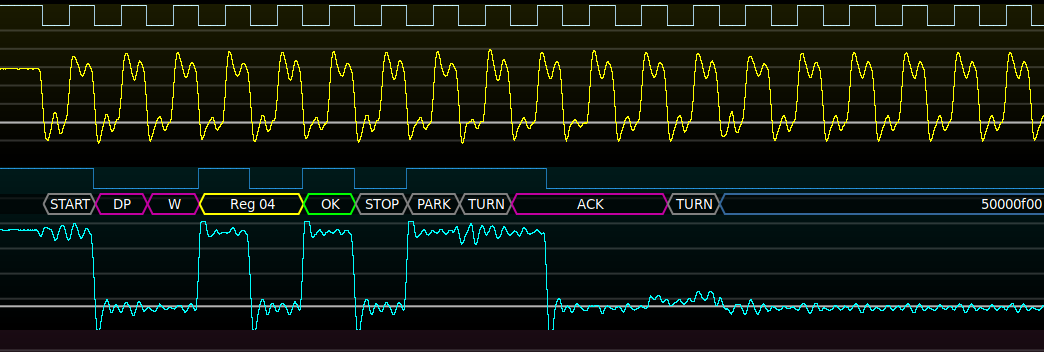
\includegraphics[width=16cm]{images/filters/swd.png}
\caption{Example of SWD protocol decode}
\label{swd_example}
\end{figure}

\subsection{Inputs}

\begin{tabularx}{16cm}{llX}
\thickhline
\textbf{Signal name} & \textbf{Type} & \textbf{Description} \\
\thickhline
SWDIO & Digital & Serial Wire Data In/Out (To/From target)\\
SWCLK & Digital & Serial Wire Clock In (To Target from Debug Probe)\\
\thickhline
\end{tabularx}

\subsection{Parameters}

No parameters are required for configuration of SWD. The protocol is clocked by SWCLK.

\subsection{Output Signal}

The SWD bus decode outputs a time series of SWD message elements, each of which may be one or a number of bits long.
Each message element consist of a type and optional numeric content.

\begin{tabularx}{16cm}{lllX}
\thickhline
\textbf{Type} & \textbf{Description} & \textbf{Color} & \textbf{Format} \\
\thickhline
Line Control & Line Reset & \cellcolor{preamble}\textcolor{white}{Preamble} & LINE RESET \\
\thickhline
Line Mode & Line Mode Change to SWD & \cellcolor{control}\textcolor{white}{Control} & JTAG TO SWD \\
\thickhline
Line Mode & Line Mode Change to JTAG & \cellcolor{control}\textcolor{white}{Control} & SWD TO JTAG \\
\thickhline
Line Mode & Line Mode Change to Dormant & \cellcolor{control}\textcolor{white}{Control} & SWD TO DORMANT \\
\thickhline
Line Mode & Leave Dormant Mode & \cellcolor{control}\textcolor{white}{Control} & LEAVE DORMANT \\
\thickhline
Start & Start of frame & \cellcolor{preamble}\textcolor{white}{Preamble} & START \\
\thickhline
APnDP & Selection between AP and DP & \cellcolor{control}\textcolor{white}{Control} & AP|DP  \\
\thickhline
RnW & Read or Write mode & \cellcolor{control}\textcolor{white}{Control} & R|W  \\
\thickhline
ADDR & AP or DP Address & \cellcolor{address}\textcolor{black}{Address} & Reg \%02x \\
\thickhline
Parity & Good Header Parity & \cellcolor{green}\textcolor{black}{Control} & OK  \\
\thickhline
Parity & Bad Header Parity & \cellcolor{red}\textcolor{white}{Control} & BAD  \\
\thickhline
Stop & End of Header & \cellcolor{preamble}\textcolor{white}{Preamble} & STOP \\
\thickhline
Park & Line Release & \cellcolor{preamble}\textcolor{white}{Preamble} & PARK \\
\thickhline
Turnaround & Line Direction Change & \cellcolor{preamble}\textcolor{white}{Preamble} & TURN \\
\thickhline
Acknowledge & Good Response from target to request & \cellcolor{control}\textcolor{white}{Control} & ACK|WAIT    \\
\thickhline
Acknowledge & Bad Response from target to request & \cellcolor{control}\textcolor{white}{Control} & FAULT|ERROR    \\
\thickhline
Data & Payload to/From Target & \cellcolor{data}\textcolor{white}{Data} & \%08x \\
\thickhline

\thickhline
\end{tabularx}

%%%%%%%%%%%%%%%%%%%%%%%%%%%%%%%%%%%%%%%%%%%%%%%%%%%%%%%%%%%%%%%%%%%%%%%%%%%%%%%%%%%%%%%%%%%%%%%%%%%%%%%%%%%%%%%%%%%%%%%%
\pagebreak
\section{SWD MEM-AP}

Converts SWD accesses to MEM-AP registers into memory read-write transactions.

Reference: ARM Debug Interface v5 Architecture Specification, chapter 8.

%%%%%%%%%%%%%%%%%%%%%%%%%%%%%%%%%%%%%%%%%%%%%%%%%%%%%%%%%%%%%%%%%%%%%%%%%%%%%%%%%%%%%%%%%%%%%%%%%%%%%%%%%%%%%%%%%%%%%%%%
\pagebreak
\section{Tachometer}

Converts pulses from a tachometer to shaft speed

%%%%%%%%%%%%%%%%%%%%%%%%%%%%%%%%%%%%%%%%%%%%%%%%%%%%%%%%%%%%%%%%%%%%%%%%%%%%%%%%%%%%%%%%%%%%%%%%%%%%%%%%%%%%%%%%%%%%%%%%
\pagebreak
\section{Tapped Delay Line}

Generic FIR filter with arbitrary tap values and delays. Can be used as-is for testing FIR filter coefficients
calculated by hand, but most commonly used as a base class for more specialized filters.

%%%%%%%%%%%%%%%%%%%%%%%%%%%%%%%%%%%%%%%%%%%%%%%%%%%%%%%%%%%%%%%%%%%%%%%%%%%%%%%%%%%%%%%%%%%%%%%%%%%%%%%%%%%%%%%%%%%%%%%%
\pagebreak
\section{TDR}

Converts a TDR waveform from volts to reflection coefficient or impedance.

%%%%%%%%%%%%%%%%%%%%%%%%%%%%%%%%%%%%%%%%%%%%%%%%%%%%%%%%%%%%%%%%%%%%%%%%%%%%%%%%%%%%%%%%%%%%%%%%%%%%%%%%%%%%%%%%%%%%%%%%
\pagebreak
\section{TDR Step De-Embed}

Given a waveform of a fast rising step, calculate the frequency response of a de-embedding network to convert the
measured waveform into an ideal unit step. The resulting data can be exported to a Touchstone file.

The calculated response is typically used as input to the de-embed filter and applied to a TDR/TDT waveform generated
with the same pulse generator. This correction allows for overshoot, ringing, and other artifacts on the pulse to be
removed from the TDR/TDT response.

It is important that the input contain a single rising edge, and is reasonably stable before and after the edge.
If multiple cycles of the test step, or falling edges, are present inaccurate results may be obtained.

NOTE: this filter is still under development and not suitable for general use.

%%%%%%%%%%%%%%%%%%%%%%%%%%%%%%%%%%%%%%%%%%%%%%%%%%%%%%%%%%%%%%%%%%%%%%%%%%%%%%%%%%%%%%%%%%%%%%%%%%%%%%%%%%%%%%%%%%%%%%%%
\pagebreak
\section{Threshold}

Converts an analog waveform to digital by thresholding at a constant level (no hysteresis).

\subsection{Inputs}

\begin{tabularx}{16cm}{llX}
\thickhline
\textbf{Signal name} & \textbf{Type} & \textbf{Description} \\
\thickhline
din & Analog & Input waveform \\
\thickhline
\end{tabularx}

\subsection{Parameters}

\begin{tabularx}{16cm}{llX}
\thickhline
\textbf{Parameter name} & \textbf{Type} & \textbf{Description} \\
\thickhline
Threshold & Float & Decision threshold \\
\thickhline
\end{tabularx}

\subsection{Output Signal}

This filter outputs an digital waveform with one sample for each sample in the input, which is true if the
corresponding input sample is above the threshold and false if less than or equal.

%%%%%%%%%%%%%%%%%%%%%%%%%%%%%%%%%%%%%%%%%%%%%%%%%%%%%%%%%%%%%%%%%%%%%%%%%%%%%%%%%%%%%%%%%%%%%%%%%%%%%%%%%%%%%%%%%%%%%%%%
\pagebreak
\section{TIE}

Calculates the time interval error of a data or clock signal with respect to an ideal ``golden" clock (typically
obtained from a CDR PLL).

%%%%%%%%%%%%%%%%%%%%%%%%%%%%%%%%%%%%%%%%%%%%%%%%%%%%%%%%%%%%%%%%%%%%%%%%%%%%%%%%%%%%%%%%%%%%%%%%%%%%%%%%%%%%%%%%%%%%%%%%
\pagebreak
\section{Top}

Calculates the top (logical one level) of each cycle in a digital waveform. It is most commonly used as an input to
statistics, to view the average top of the entire waveform.

\subsection{Inputs}

\begin{tabularx}{16cm}{llX}
\thickhline
\textbf{Signal name} & \textbf{Type} & \textbf{Description} \\
\thickhline
din & Analog & Input waveform \\
\thickhline
\end{tabularx}

\subsection{Parameters}

This filter takes no parameters.

\subsection{Output Signal}

This filter outputs an analog waveform with one sample for each group of logical ones in the input signal, containing
the average value of the one level.

%%%%%%%%%%%%%%%%%%%%%%%%%%%%%%%%%%%%%%%%%%%%%%%%%%%%%%%%%%%%%%%%%%%%%%%%%%%%%%%%%%%%%%%%%%%%%%%%%%%%%%%%%%%%%%%%%%%%%%%%
\pagebreak
\section{Touchstone Import}

Loads a Touchstone file and displays the complex data in magnitude/angle format

%%%%%%%%%%%%%%%%%%%%%%%%%%%%%%%%%%%%%%%%%%%%%%%%%%%%%%%%%%%%%%%%%%%%%%%%%%%%%%%%%%%%%%%%%%%%%%%%%%%%%%%%%%%%%%%%%%%%%%%%
\pagebreak
\section{UART}

%%%%%%%%%%%%%%%%%%%%%%%%%%%%%%%%%%%%%%%%%%%%%%%%%%%%%%%%%%%%%%%%%%%%%%%%%%%%%%%%%%%%%%%%%%%%%%%%%%%%%%%%%%%%%%%%%%%%%%%%
\pagebreak
\section{USB 1.0 / 2.x Activity}

%%%%%%%%%%%%%%%%%%%%%%%%%%%%%%%%%%%%%%%%%%%%%%%%%%%%%%%%%%%%%%%%%%%%%%%%%%%%%%%%%%%%%%%%%%%%%%%%%%%%%%%%%%%%%%%%%%%%%%%%
\pagebreak
\section{USB 1.0 / 2.x Packet}

%%%%%%%%%%%%%%%%%%%%%%%%%%%%%%%%%%%%%%%%%%%%%%%%%%%%%%%%%%%%%%%%%%%%%%%%%%%%%%%%%%%%%%%%%%%%%%%%%%%%%%%%%%%%%%%%%%%%%%%%
\pagebreak
\section{USB 1.0 / 2.x PCS}

%%%%%%%%%%%%%%%%%%%%%%%%%%%%%%%%%%%%%%%%%%%%%%%%%%%%%%%%%%%%%%%%%%%%%%%%%%%%%%%%%%%%%%%%%%%%%%%%%%%%%%%%%%%%%%%%%%%%%%%%
\pagebreak
\section{USB 1.0 / 2.x PMA}

%%%%%%%%%%%%%%%%%%%%%%%%%%%%%%%%%%%%%%%%%%%%%%%%%%%%%%%%%%%%%%%%%%%%%%%%%%%%%%%%%%%%%%%%%%%%%%%%%%%%%%%%%%%%%%%%%%%%%%%%
\pagebreak
\section{Undershoot}

%%%%%%%%%%%%%%%%%%%%%%%%%%%%%%%%%%%%%%%%%%%%%%%%%%%%%%%%%%%%%%%%%%%%%%%%%%%%%%%%%%%%%%%%%%%%%%%%%%%%%%%%%%%%%%%%%%%%%%%%
\pagebreak
\section{Upsample}

Upsamples a waveform using sin(x)/x interpolation.

%%%%%%%%%%%%%%%%%%%%%%%%%%%%%%%%%%%%%%%%%%%%%%%%%%%%%%%%%%%%%%%%%%%%%%%%%%%%%%%%%%%%%%%%%%%%%%%%%%%%%%%%%%%%%%%%%%%%%%%%
\pagebreak
\section{Vector Frequency}
\label{filter:vector_frequency}

Calculates the instantaneous frequency (rotational velocity) of a complex I/Q signal.

%%%%%%%%%%%%%%%%%%%%%%%%%%%%%%%%%%%%%%%%%%%%%%%%%%%%%%%%%%%%%%%%%%%%%%%%%%%%%%%%%%%%%%%%%%%%%%%%%%%%%%%%%%%%%%%%%%%%%%%%
\pagebreak
\section{Vector Phase}

Calculates the instantaneous phase of a complex I/Q signal.

%%%%%%%%%%%%%%%%%%%%%%%%%%%%%%%%%%%%%%%%%%%%%%%%%%%%%%%%%%%%%%%%%%%%%%%%%%%%%%%%%%%%%%%%%%%%%%%%%%%%%%%%%%%%%%%%%%%%%%%%
\pagebreak
\section{Vertical Bathtub}

%%%%%%%%%%%%%%%%%%%%%%%%%%%%%%%%%%%%%%%%%%%%%%%%%%%%%%%%%%%%%%%%%%%%%%%%%%%%%%%%%%%%%%%%%%%%%%%%%%%%%%%%%%%%%%%%%%%%%%%%
\pagebreak
\section{Waterfall}

%%%%%%%%%%%%%%%%%%%%%%%%%%%%%%%%%%%%%%%%%%%%%%%%%%%%%%%%%%%%%%%%%%%%%%%%%%%%%%%%%%%%%%%%%%%%%%%%%%%%%%%%%%%%%%%%%%%%%%%%
\pagebreak
\section{WAV Import}

Loads waveform data from a Microsoft WAV audio file.

%%%%%%%%%%%%%%%%%%%%%%%%%%%%%%%%%%%%%%%%%%%%%%%%%%%%%%%%%%%%%%%%%%%%%%%%%%%%%%%%%%%%%%%%%%%%%%%%%%%%%%%%%%%%%%%%%%%%%%%%
\pagebreak
\section{Windowed Autocorrelation}

Calculates the cross-correlation between a fixed size block of the input signal and another block of the same size.

This will produce maximal response for a signal which has periodicity with the specified period and block size.

For example, period 4 and block size 2 will match aa**aa**.

This can be used to identify OFDM symbols.
